\documentclass[12pt,oneside,a4paper]{article}

\usepackage[left=1in, top=1.5in, right=1in, bottom=1.2in]{geometry}

\usepackage[style=numeric]{biblatex}
\usepackage{xcolor}
\usepackage{amsmath, amssymb}
\usepackage{multicol}
\usepackage{caption}
\usepackage{hyperref}
\usepackage{graphicx}
\usepackage{listings}
\usepackage{tabularx}
\usepackage{ltablex}
\usepackage{booktabs}

\pagestyle{headings}

\addbibresource{biblio.bib}

\title{Formal Methods for Concurrent and Real-Time Systems}
\author{Giacomini Davide \and Giarduz Andrea \and Grosso Veronica}

\newcommand{\UPPAAL}{{\scshape Uppaal}}

\begin{document}
\begin{titlepage}
\begin{center}
        \vspace*{-1,5cm}
		
\includegraphics[width=5cm]{resources/logo.png}
		
        \LARGE{{\scshape Politecnico di Milano}}
        
        \LARGE{}
        
        \LARGE{2020/2021}
        
        \vspace*{1cm}
        \Large{{\scshape Formal Methods for Concurrent and Real-Time Systems}}
        
        \vspace*{1cm}
        \Huge{\textbf{Model Checking of Warehouse Robotics}}
 
 		\Large{Homework Project Report}
        \vfill
        
        \vspace*{0,8cm}
        \Large{{\scshape Authors} \\ Giacomini Davide\\
        Giarduz Andrea\\
        Grosso Veronica
        }
            
        \vspace{1,2cm}
           
        \Large
        {\scshape Instructors}\\
        Prof. San Pietro Pierluigi\\
        Dr. Lestingi Livia
    \end{center}
\end{titlepage}

\pagenumbering{Roman}
\setcounter{tocdepth}{3}
\tableofcontents
\listoffigures
\addcontentsline{toc}{section}{\listfigurename}
\listoftables
\addcontentsline{toc}{section}{\listtablename}

\newpage
\pagenumbering{arabic}

\begin{abstract}\addcontentsline{toc}{section}{Abstract}
The development of cutting-edge technologies in automated warehouses has taken outstanding steps in the last few years. 
This fast-paced environment requires a high level of reliability, in terms of speed and interaction between the many system components.
Formal verification plays an essential role in ensuring an error-free environment, by analysing synthetic models, that capture the main features of the real-world problem.\\
The Model Checking of Warehouse Robotics project employs \UPPAAL\ \cite{uppaal} to model a simplified automated warehouse environment. The goal is to verify some significant properties in different scenarios, in order to show the correctness of the model.
\end{abstract}

\section{Introduction}
The Model Checking of Warehouse Robotics project is divided in two main focus areas: first, the efforts are placed in modelling the environment; then the target becomes the verification of significant properties, applied to the aforementioned model.

The goal is the handling of multiple tasks: each task contains the information about a specific item (placed in a pod inside the warehouse) that needs to be delivered. 
In particular, the high level model consists in a set of three different components, specifically the human, the robots and the task queue generator.
The environment where these components interact is a rectangular grid (i.e., the warehouse floor plan). It is possible to identify on the map an entry point, a delivery point and a set of pods.

\begin{tabularx}{\textwidth}{lX}
\textbf{Entry point} & It is the initial slot where all the robots are placed at the beginning of the simulation.\vspace{0,2cm}\\
\textbf{Delivery point} & It is the slot where the items need to be delivered.\vspace{0,2cm}\\
\textbf{Pod} & It includes some items and it can be moved by the robots.\vspace{0,2cm}\\
\end{tabularx}

\noindent Specifically, these are the main features of the components:
\vspace{0,5cm}

\begin{tabularx}{\textwidth}{lX}
\textbf{Human} & The job of the operator is to pick up an item once a robot comes into the human working station. The operator is kept by default at the edge of the system.\vspace{0,2cm}\\
\textbf{Robot} & It is in charge of the delivery of a specific pod to a human, according to what specified in a task.\vspace{0,2cm}\\
\textbf{Task queue} & It periodically generates new tasks and places them into a First-In-First-Out (FIFO) queue.\vspace{0,2cm}\\
\end{tabularx}

Non-deterministic delays in the actions performed by the components have been included in order to create a model closer to a real-world situation, using \UPPAAL SMC.
\section{Component Description}
The detailed description of the system components is presented in this section. It is comprehensive of the mandatory features and behavioural aspects, the simplifying assumptions and the rationale behind the adopted choices.

\subsection{Environment and System Declarations}
The project declarations contain the auxiliary functions and variables to facilitate the implementation of the model. 
For instance, functions such as \texttt{stdNormal()} and \texttt{Normal(mean, stdDev)} are essential to produce the delays that follow a Normal Distribution.

Moreover, this section features the constants and, in a more general way, the required data structures. The most important characteristics are:

\begin{tabularx}{\textwidth}{lX}
\textbf{Grid} & The warehouse floor plan has been represented by a parametric N $\times$ M matrix. The matrix choice easily allows to compute offsets and distances between grid slots. Furthermore it has an intuitive visual prospect.

The grid layout is flexible and can be changed by setting the N, M values, the pods positions, as well as the entry and delivery points. In Figure \ref{fig:grid10x10} it is possible to see an example of a grid layout. \vspace{0,2cm}\\
\textbf{Pods} & The pods id, position and status are saved in a matrix \texttt{pods[PODS\_N][3]}, where \texttt{PODS\_N} is the total number of pods. The first index is the pod id, while the second one contains the x and y coordinates and the pod status. The pods can either be free or assigned to a task. 

This data structure allows an easy access to both the position and status of pods by their id.\vspace{0,2cm}\\
\textbf{Queue} & It is a FIFO array, of size \texttt{MAX\_T}, containing the pending tasks. The parameter \texttt{MAX\_T} represents the maximum queue size. Together with the \texttt{current\_length\_queue} variable, it is possible to model a queue variable in length, despite \UPPAAL \ not providing dynamic memory management. \vspace{0,2cm}\\
\end{tabularx}

\begin{figure}
    \centering
    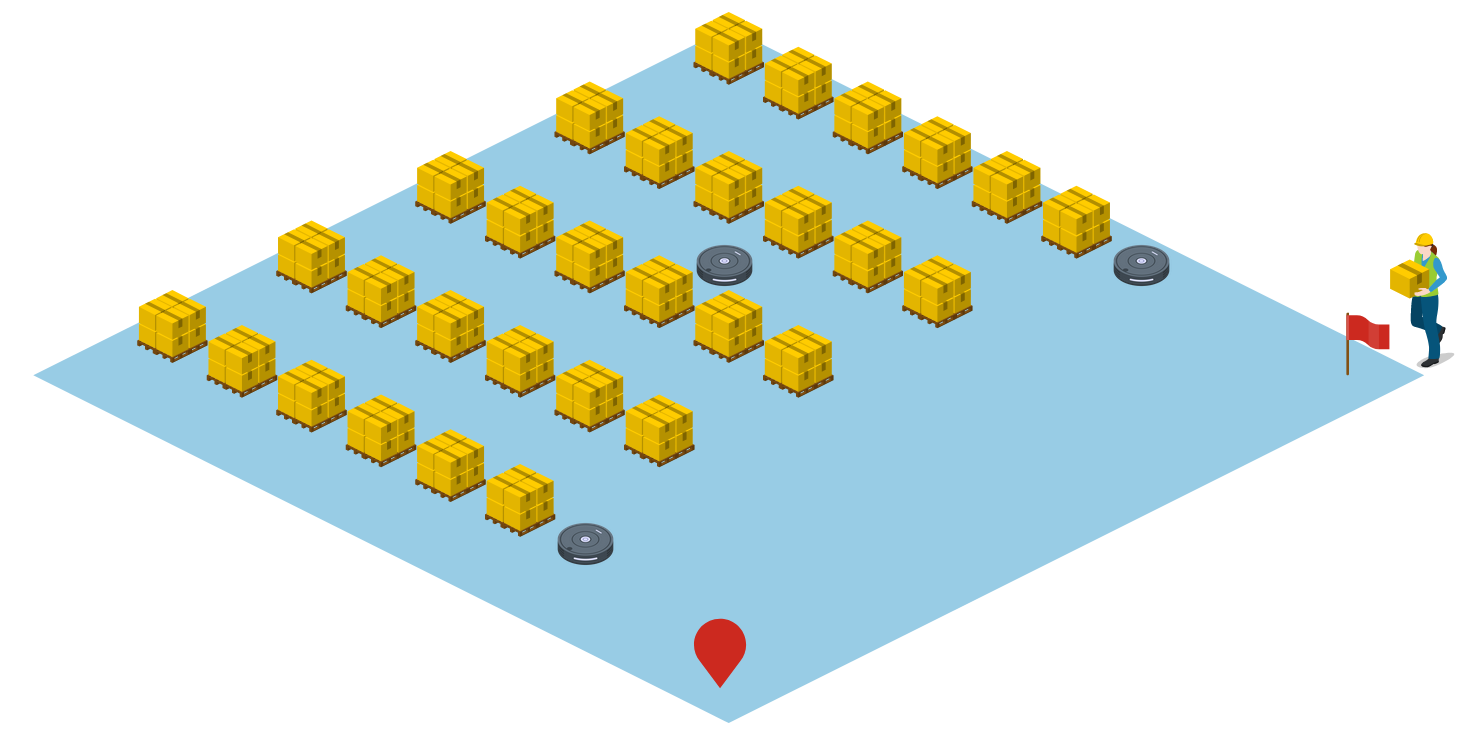
\includegraphics[width=0.75\textwidth]{resources/grid10x10.png}
    \caption{Example of a grid layout}
    \label{fig:grid10x10}
\end{figure}

\subsection{Task Queue}
The Task Queue template models the generation and dispatching of tasks. Since this is the first entity to start the computation, it initializes the grid, the pods and the queue. 

\begin{tabularx}{\textwidth}{lX}
\multicolumn{2}{l}{{\scshape Normal Execution}}
 \vspace{0,2cm}\\
\texttt{task\_generation} & The Task Queue generates a new task and places it in the FIFO queue. The generation happens with a variable delay \texttt{task\_delay}, computed every time following a Normal Distribution \cite{David2015}. \vspace{0,2cm}\\
\texttt{task\_sent} & The timed automaton synchronizes with an idle robot on the first item of the task queue. It sends the information about the pod id, matched with the task, to the robot. After that, it removes the assigned task from the queue. This is useful because it avoids that multiple robots process the same task. \vspace{0,4cm}\\
\multicolumn{2}{l}{{\scshape Error States}} \vspace{0,2cm}\\
\texttt{Error\_maxSizeReached}  & This error state is reached when the task queue is full. The newly generated tasks would be lost, so the timed automaton stops its behaviour. \vspace{0,2cm}\\
\texttt{Err\_podsUnavailable}   & The pods unavailable error state happens whenever the number of tasks overcomes the number of available pods. In particular, the new tasks cannot be associated with any pod, creating an undesired situation. Naturally, for this to happen, \texttt{MAX\_T} $>$ \texttt{PODS\_N} must hold. \vspace{0,2cm}\\
\end{tabularx}

\subsection{Robots}
The Robot template is the most complex component in the system, since it handles the task retrieval, the robot movement algorithm, the pod delivery and the returning of the pod to its original position.
In order to do so, it synchronizes both with the Task Queue and the Human Operator. 

The key feature in this automaton is that the states represent ongoing actions (e.g., reaching a pod, going to the delivery point, etc.), that are gradually executed with the self-loop transitions. This way, the model is kept as simple as possible, by avoiding to insert intermediate states. \\
Transition between different states, on the other hand, are related to different phases of the robot activity (e.g., the pod has been delivered, so the destination of the robot changes). Thus, the model has a constant structure. 
The idle position, \texttt{start}, features an exponential delay, which could represent a non-deterministic robot behaviour in the processing before taking a new task.

\subsection{Human Operator}	
The Human Operator is modelled as a two-state timed automaton, to make it as simple as possible. As soon as a robot arrives in the delivery point with a pod, it synchronizes with the operator. The human picks up the right item from the pod. It takes the human with a delay \texttt{human\_delay} modelled by a Normal Distribution. When the job is done, it notifies the robot that it is free to go. 

\subsection{Design Choices}
The main design choices and assumptions for this project can be summarized into four main areas:

\begin{tabularx}{\textwidth}{lX}
\textbf{Robot movement} & In order to keep the verification times short, while using an efficient movement algorithm, we chose to suppose to existence of a \textit{robot highway} on the right side of the map, containing the entry and delivery points. The algorithm works by preferring a tile with the minimum Manhattan distance to the destination. The choice of the Manhattan distance is due to the robot not being able to move diagonally. The preferred direction, at this point, is moving towards the \textit{robot highway}, hence the assumption on its existence. This way, robots are less prone to routing congestion. If possible, the robot tries not to move to the tile it previously occupied. This avoids starving conditions where two robots keep performing the same movements over and over again. Because of these design choices, the algorithm works best with horizontal alternated parallel lanes of pods. \vspace{0,2cm}\\
\textbf{States number} & The target of the modelling phase for each template was to keep the number of states low, thus allowing a faster verification and a better readability. \vspace{0,2cm}\\
\textbf{Channel policy} & The \UPPAAL \ SMC extension requires all channels to be \texttt{broadcast}. In our model, this is not a problem, since communication is ensured to be one-to-one. The only relevant point where this could have been an issue is the \texttt{free\_robot} channel, as the others have only one possible receiver (either the Task Queue or the Human Operator). In spite of this, only one robot can occupy the delivery point, hence only the rightful synchronization will be activated. \vspace{0,2cm}\\
\textbf{New task selection} & A reduction of complexity also took place in the policy of new task selection. A number $n \in \left[0,\texttt{PODS\_N}\right] $ is randomly chosen by the tool. In order to find the first available pod, we compute $ m = n \mod \texttt{free\_pods\_number()} $, and then we search the $m$-th free pod in the pods status array. This ensures to always find a free pod, no matter the value of $n$ chosen by \UPPAAL . \vspace{0,2cm}\\
\end{tabularx}
\section{Properties}

\subsection{Property description}

\subsection{Application of the properties}

\subsubsection{First Scenario}


\subsubsection{Second Scenario}
\section{Conclusions}
In this report, we presented an analysis of the problem of the Model Checking of Warehouse Robotics. The scrutiny was focused on both realistic configurations and stressed configurations, in order to understand the validity of the representation of the system. To sum up, the model appears coherent with the specifications of the project and with abstract real-life situations.

\printbibliography\addcontentsline{toc}{section}{References}

\end{document}
